
\begin{frame}
  \frametitle{L'API OpenGL du point vue du codeur C}
  \begin{textblock}{12}(12,1.25)
    \begin{tikzpicture}
      % \draw [help lines] grid(3,2);
      % \pgfuseimage{FunnyPythonSmall}
      \node[inner sep=0pt] at (0,0) {
\includegraphics[height=10mm]{images/funny-python.png}};
      \node[draw=black, cloud callout, cloud puffs=15, aspect=2.5, cloud puff arc=120,
      callout relative pointer={(-.6,-.3)}] at (1.5,1) {void \ptr\ptr}; % absolute fails ?
    \end{tikzpicture}
  \end{textblock}
  % \frametitle{Présentation de l'API OpenGL}
  % titre ?
  API OpenGL V4.5 core~: % {\tiny (compatibility)}
  \begin{itemize}
  \item 1328 constantes {\small i.e.\ 0x1234} % {\tiny (1757)}
  \item 653 fonctions \\[.5em] % {\tiny (1044)} 
  \end{itemize}
  Paramètres~:
  \begin{itemize}
  \item type de base via typedef~: \code{(unsigned) char, short, int, float, double}
  \item pointeur~: \code{void \ptr(\ptr), char \ptr(\ptr), int \ptr, float \ptr, \ldots} \\[.5em] % * glyph
  \end{itemize}
  Return~:
  \begin{itemize}
  \item \code{unsigned char, (unsigned) int}
  \item \code{void \ptr, const unsigned char \ptr} {\tiny (quelques cas)}
  \end{itemize}
\end{frame}

\begin{frame}[fragile]
  \frametitle{XML API Registry~:  c'est cool!}
  \begin{tikzpicture}[remember picture, overlay, mystyle/.style={fill=red!20, opacity=1.}] % run twice
    \fill[mystyle] ($(current page.south west) + (2.4,3.3)$) rectangle +(3.2,.5);
    \node [mystyle, rectangle callout, callout relative pointer={(-3.5,-.5)}]
    at ($(current page.south west) + (10,4.5)$) {la taille est indiqué};
  \end{tikzpicture}
  \href{https://www.opengl.org/registry}{Fichier XML} définissant~: \\
  \begin{itemize}
    \item les constantes
    \item les fonctions et leurs prototypes \\
      {\tiny%
\begin{verbatim}
void glClearBufferData (GLenum target, GLenum internalformat, GLenum format, GLenum type, const void * data)

<command>
    <proto>void <name>glClearBufferData</name></proto>
    ...
    <param><ptype>GLenum</ptype> <name>format</name></param>
    <param><ptype>GLenum</ptype> <name>type</name></param>
    <param len="COMPSIZE(format,type)">const void *<name>data</name></param>
</command>
\end{verbatim}}
    \item les extensions
    \item les \textbf{versions} et leurs \textbf{profiles}
  \end{itemize}
  \centerline{\alert{$\longrightarrow$ Apporte des informations essentielles par rapport au fichier d'en-tête}}
\end{frame}

\begin{frame}
  \frametitle{Architecture}
  \begin{center}
    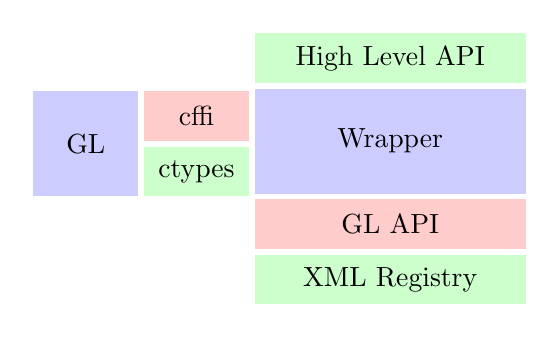
\begin{tikzpicture}[%
      base/.style={rectangle, minimum width=10em, minimum height=2em, anchor=south west,
        draw=white, line width=2pt},
      double/.style={base, minimum height=4em},
      small/.style={base, minimum width=4em, anchor=east}]
      % \draw [help lines] grid(3,2);
      \node[base, fill=green!20] at (0,0) {XML Registry};
      \node[base, fill=red!20] at (0,2em) {GL API};
      \node[double, fill=blue!20] at (0,4em) {Wrapper};
      \node[small, fill=green!20] at (2pt,5em) {ctypes}; % 2pt ???
      \node[small, fill=red!20] at (2pt,7em) {cffi};
      \node[double, minimum width=4em, anchor=east, fill=blue!20] at (-4em+2pt,6em) {GL};
      \node[base, fill=green!20] at (0,8em) {High Level API};
    \end{tikzpicture}
  \end{center}
\end{frame}

\begin{frame}
  \frametitle{Les prototypes de fonctions en C}
  \begin{itemize}
    \item principe de base~: \\
      \code{output\_type function(type parameter, \ldots)}
    \item plus d'une valeur retournée~: \\
      \code{output\_type function(type \alert{\ptr} parameter, \ldots)}
    \item transmettre des tableaux~: \\
      \code{output\_type function(size\_type size, data\_type \ptr array, \ldots)}
    \item transmettre des tableaux en lecture seul~: \\
      \code{output\_type function(size\_type size, \alert{const} data\_type \ptr array, \ldots)}
  \end{itemize}
\end{frame}

\begin{frame}
  \frametitle{Tous les paramètres ne ressemblent pas \ldots}
  \begin{description}[input/output via pointeur]
    \item[simple] \texttt{GLenum target}
    \item[output par référence] \texttt{int \colorR{\ptr [1]} length}
      % plus d'un paramètre retourné
    \item[input via pointeur] \texttt{GLsizeiptr size, \colorR{const} void \colorR{\ptr [size]} data}
    \item[input/output via pointeur] \texttt{GLsizeiptr size, void \colorR{\ptr [size]} data}
    \item[pointeur complexe] \texttt{GLenum pname, GLint \colorR{\ptr [COMPSIZE(pname)]} data} \\
      \texttt{const void \ptr [COMPSIZE(format,type,width)] pixels}
  \end{description}
\end{frame}

\begin{frame}
  \frametitle{Tous les paramètres ne ressemblent pas \ldots}
  \begin{description}[input/output via pointeur]
    \item[simple] \texttt{GLenum target} \\
      \colorB{Python $\longrightarrow$ C}
    \item[output par référence] \texttt{int \alert{\ptr [1]} length} \\
      \colorB{%
        disparaît du prototype Python \\
        C  $\longrightarrow$ Python \\
        retourné dans l'ordre d'apparition \\[.5em]
        \colorbox{\bgR}{int} foo(\colorbox{green!20!white}{int p1}, \colorbox{blue!20!white}{int \ptr r1, int \ptr r2}) \\
        % $\longrightarrow$ \\
        \colorbox{red!20!white}{o0}, \colorbox{blue!20!white}{r1, r2} = foo(\colorbox{green!20!white}{p1})
      }
  \end{description}
\end{frame}

\begin{frame}
  \frametitle{Tous les paramètres ne ressemblent pas \ldots}
  \begin{description}[input/output via pointeur]
    \item[input via pointeur] \texttt{GLsizeiptr size, \colorR{const} void \colorR{\ptr [size]} data} \\
      %\colorB{%
        pointeur disparaît du prototype Python \\
        \texttt{size = len(p)} \\
        \begin{tikz}
          \node [fill=yellow!80, isosceles triangle, shape border rotate=90, inner sep=.1pt, rounded corners] {!};
        \end{tikz}%
        \alert{XML est incomplet: size = len(p) or size\_of(p)} \\
        logiquement \texttt{void} $\Longrightarrow$ \texttt{size\_of} et \texttt{float} $\Longrightarrow$ \texttt{len}
        \begin{enumerate}
          \item type = \texttt{const char \ptr\ptr}~: \texttt{str(p)} ou \texttt{[str(x) for x in p]}
          \item p = Numpy array~: check type if type not void
          \item p = iterable
        \end{enumerate}
        int foo(int p1, int \ptr s2, float \ptr p2) \\
        $\longrightarrow$ \\
        o0 = foo(p1, p2)
      %}
  \end{description}
\end{frame}

\begin{frame}
  \frametitle{Input/Output via Pointeur}
  \begin{enumerate}
  \item type = \texttt{void \ptr}~: p = Numpy array, \texttt{size = p.nbytes} \\
    int foo(int p1, int \ptr s2, float \ptr p2) \\
    $\longrightarrow$ \\
    o0 = foo(p1, p2)
    % 
  \item type = \texttt{char \ptr}~: p = size, new string \\
    int foo(int p1, int \ptr s2, char \ptr p2) \\
    $\longrightarrow$ \\
    o0, p2 = foo(p1, s2)
    % 
  \item p = Numpy array~: check type, \texttt{size = p.size} \\
    idem \texttt{void \ptr}
    % 
  \item p = size~: return a Numpy array or list \\
    idem \texttt{char \ptr}
  \end{enumerate}
\end{frame}

\begin{frame}
  \frametitle{Pointeur Complexe}
  \begin{enumerate}
    \setbeamercolor{item projected}{bg=blue!50!white,fg=white}
  \setbeamertemplate{enumerate items}[circle]
  \item type = \texttt{const char \ptr}
  \item p = Numpy array~: check type if type not void
  \end{enumerate}
\end{frame}

%%% Local Variables: 
%%% mode: latex
%%% TeX-master: "master"
%%% End: 
